% Copyright 2005-2016 Airbus-EDF-IMACS-Phimeca
% Permission is granted to copy, distribute and/or modify this document
% under the terms of the GNU Free Documentation License, Version 1.2
% or any later version published by the Free Software Foundation;
% with no Invariant Sections, no Front-Cover Texts, and no Back-Cover
% Texts.  A copy of the license is included in the section entitled "GNU
% Free Documentation License".
\renewcommand{\etapemethodo}{B}
\renewcommand{\nomfichier}{docref_B234_LinearRegression}
\renewcommand{\titrefiche}{Linear regression}

\Header

\MathematicalDescription{

  \underline{\textbf{Goal}} \vspace{2mm}

  This method deals with the parametric modelling of a probability distribution for a random vector $\vect{X} = \left( X^1,\ldots,X^{n_X} \right)$. It aims to measure a type of dependence (here a linear relation) which may exist between a component $X^i$ and other uncertain variables $X^j$.
  \vspace{2mm}

  \underline{\textbf{Principle of the method}} \vspace{2mm}

  The principle of the multiple linear regression model is to find the function that links the variable $X^i$ to other variables $X^{j_1}$,\ldots,$X^{j_K}$ by means of a linear model:
  \begin{align*}
    X^i = a_0 + \sum_{j \in \{ j_1,\ldots,j_K \} } a_j X^j + \varepsilon
  \end{align*}
  where $\varepsilon$ describes a random variable with zero mean and standard deviation $\sigma$ independent of the input variables $X^i$. For given values of $X^{j_1}$,\ldots,$X^{j_K}$, the average forecast of $X^i$ is denoted by $\widehat{X}^i$ and is defined as:
  \begin{align*}
    \widehat{X}^i = a_0 + \sum_{j \in \{ j_1,\ldots,j_K \} } a_j X^j
  \end{align*}

  The estimators for the regression coefficients $\widehat{a}_0,\widehat{a}_1,\ldots,\widehat{a}_{K}$, and the standard deviation $\sigma$ are obtained from a sample of $(X^i,X^{j_1},\ldots,X^{j_K})$, that is a set of $N$ values $(x^i_1,x_1^{j_1},\ldots,x_1^{j_K})$,\ldots,$(x^i_n,x_n^{j_1},\ldots,x_n^{j_K})$. They are determined via the least-squares method:

  \begin{align*}
    \left\{ \widehat{a}_0,\widehat{a}_1,\ldots,\widehat{a}_{K} \right\} = \textrm{argmin} \sum_{k=1}^n \left[ x^i_k - a_0 - \sum_{j \in \{ j_1,\ldots,j_K \} } a_j x^j_k \right]^2
  \end{align*}

  In other words, the principle is to minimize the total quadratic distance between the observations $x^i_k$ and the linear forecast $\widehat{x}^i_k$.

  Some estimated coefficient $\widehat{a}_\ell$ may be close to zero, which may indicate that the variable $X^{j_\ell}$ does not bring valuable information to forecast $X^i$. OpenTURNS includes a classical statistical test to identify such situations: Fisher's test.  For each estimated coefficient $\widehat{a}_\ell$, an important characteristic is the so-called "$p$-value" of Fisher's test. The coefficient is said to be "significant" if and only if $\alpha_{\ell \textrm{lim}}$ is greater than a value $\alpha$ chosen by the user (typically 5\% or 10\%). The higher the $p$-value, the more significant the coefficient.

  Another important characteristic of the adjusted linear model is the coefficient of determination $R^2$. This quantity indicates the part of the variance of $X^i$ that is explained by the linear model:
  \begin{align*}
    R^2 = \frac{ \displaystyle \sum_{k=1}^n \left( x^i_k - \overline{x}^i \right)^2 - \sum_{k=1}^n \left( x^i_k - \widehat{x}_k^i \right)^2 }{ \sum_{k=1}^n \left( x^i_k - \overline{x}^i \right)^2 }
  \end{align*}
  where $\overline{x}^i$ denotes the empirical mean of the sample $\left\{ x^i_1,\ldots,x^i_n  \right\}$.

  Thus, $0 \leq R^2 \leq 1$. A value close to 1 indicates a good fit of the linear model, whereas a value close to 0 indicates that the linear model does not provide a relevant forecast. A statistical test allows to detect significant values of $R^2$. Again, a $p$-value is provided: the higher the $p$-value, the more significant the coefficient of determination.

  By definition, the multiple regression model is only relevant for linear relationships, as in the following simple example where $X^2 = a_0 + a_1 X^1$.

  \begin{center}
    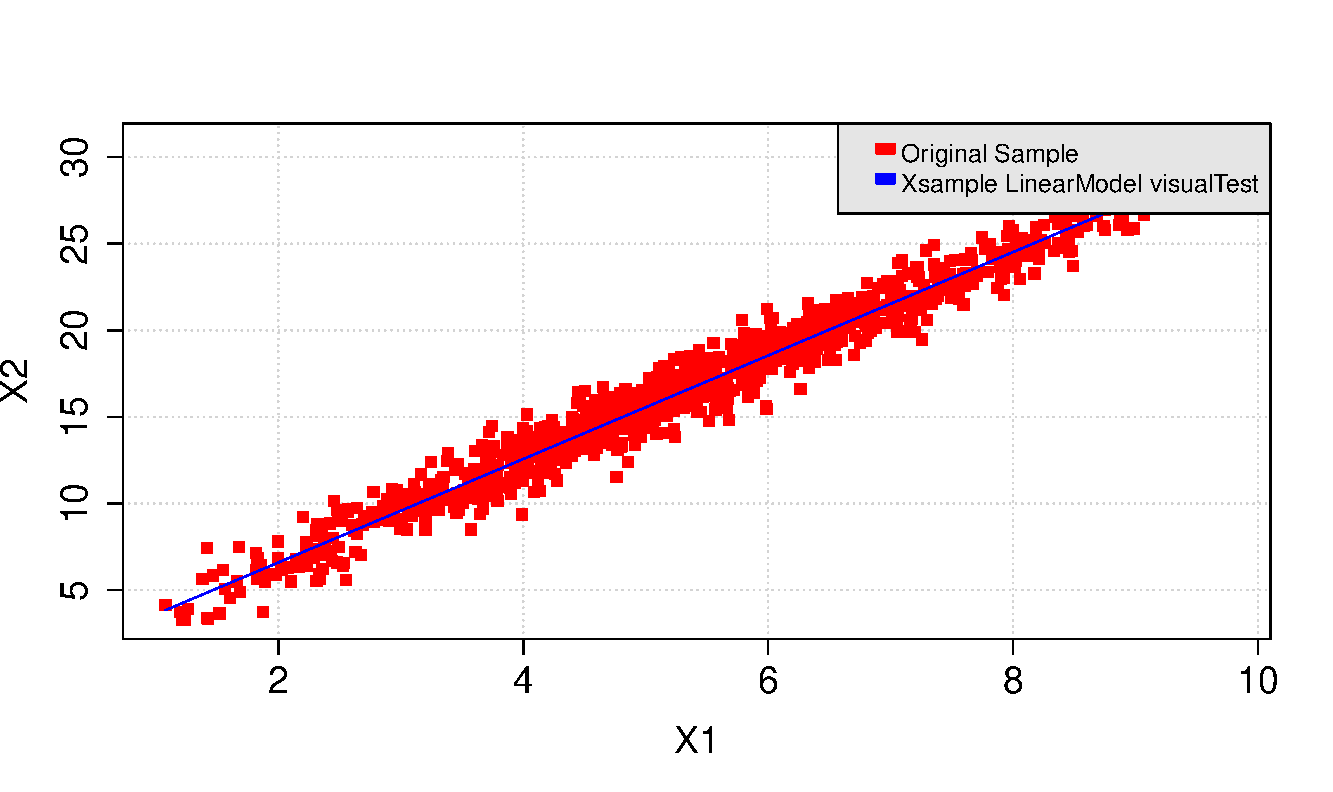
\includegraphics[scale=0.45]{Figures/OKlinearRegModel.pdf}
  \end{center}

  In this second example (still in dimension 1), the linear model is not relevant because of the exponential shape of the relation. But a linear approach would be useful on the transformed problem $X^2 = a_0 + a_1 \exp X^1$. In other words, what is important is that the relationships between $X^i$ and the variables $X^{j_1}$,\ldots,$X^{j_K}$ is linear with respect to the regression coefficients $a_j$.

  \begin{center}
    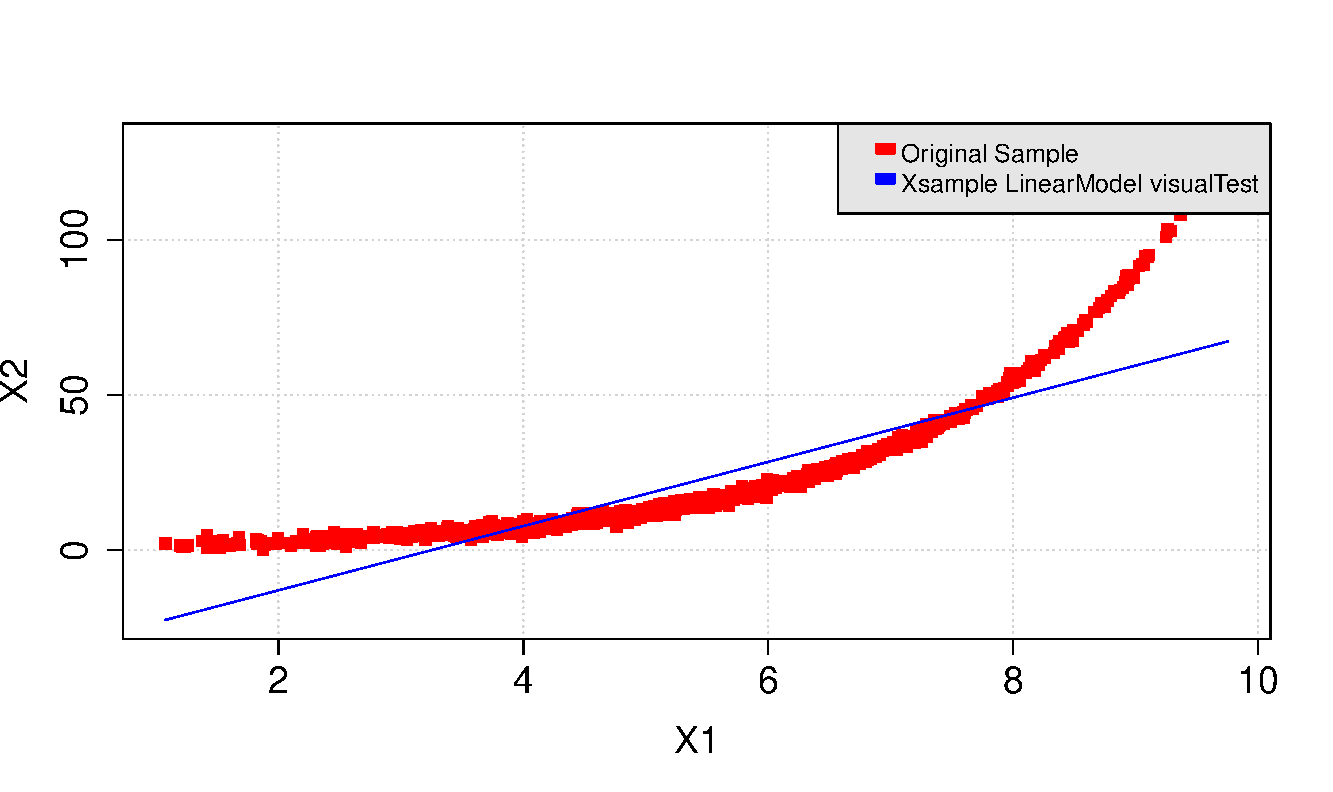
\includegraphics[scale=0.45]{Figures/WronglinearRegModel.pdf}
  \end{center}

  The value of $R^2$ is a good indication of the goodness-of fit of the linear model. However, several other verifications have to be carried out before concluding that the linear model is satisfactory. For instance, one has to pay attentions to the "residuals" $\{ u_1,\ldots,u_N \} $ of the regression:
  \begin{align*}
    u_j = x^i - \widehat{x}^i
  \end{align*}
  A residual is thus equal to the difference between the observed value of $X^i$ and the average forecast provided by the linear model. A key-assumption for the robustness of the model is that the characteristics of the residuals do not depend on the value of $X^i,X^{j_1}$,\ldots,$X^{j_K}$: the mean value should be close to 0 and the standard deviation should be constant. Thus, plotting the residuals versus these variables can fruitful.

  In the following example, the behaviour of the residuals is satisfactory: no particular trend can be detected neither in the mean nor in he standard deviation.

  \begin{center}
    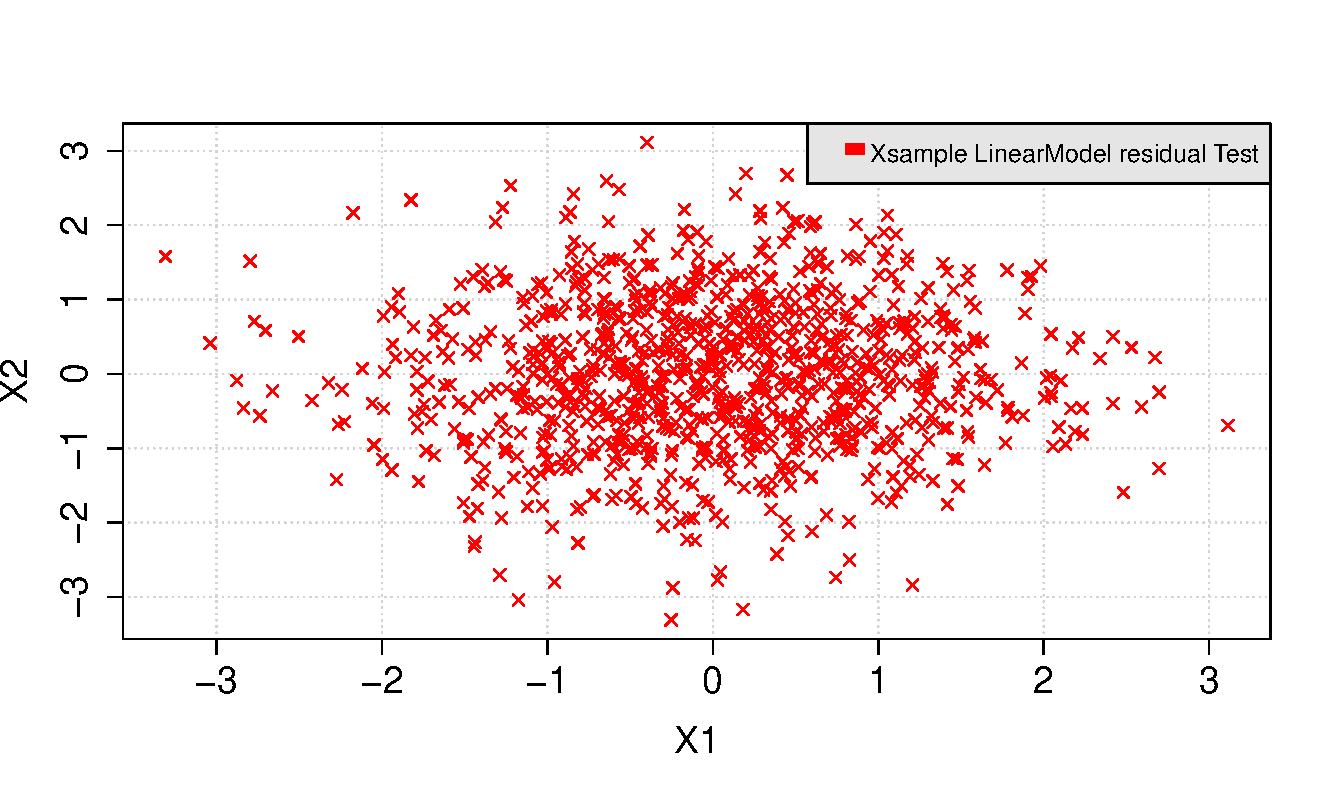
\includegraphics[scale=0.45]{Figures/OKlinearRegModelResidual.pdf}
  \end{center}

  The next example illustrates a less favourable situation: the mean value of the residuals seems to be close to 0 but the standard deviation tends to increase with $X$. In such a situation, the linear model should be abandoned, or at least used very cautiously.

  \begin{center}
    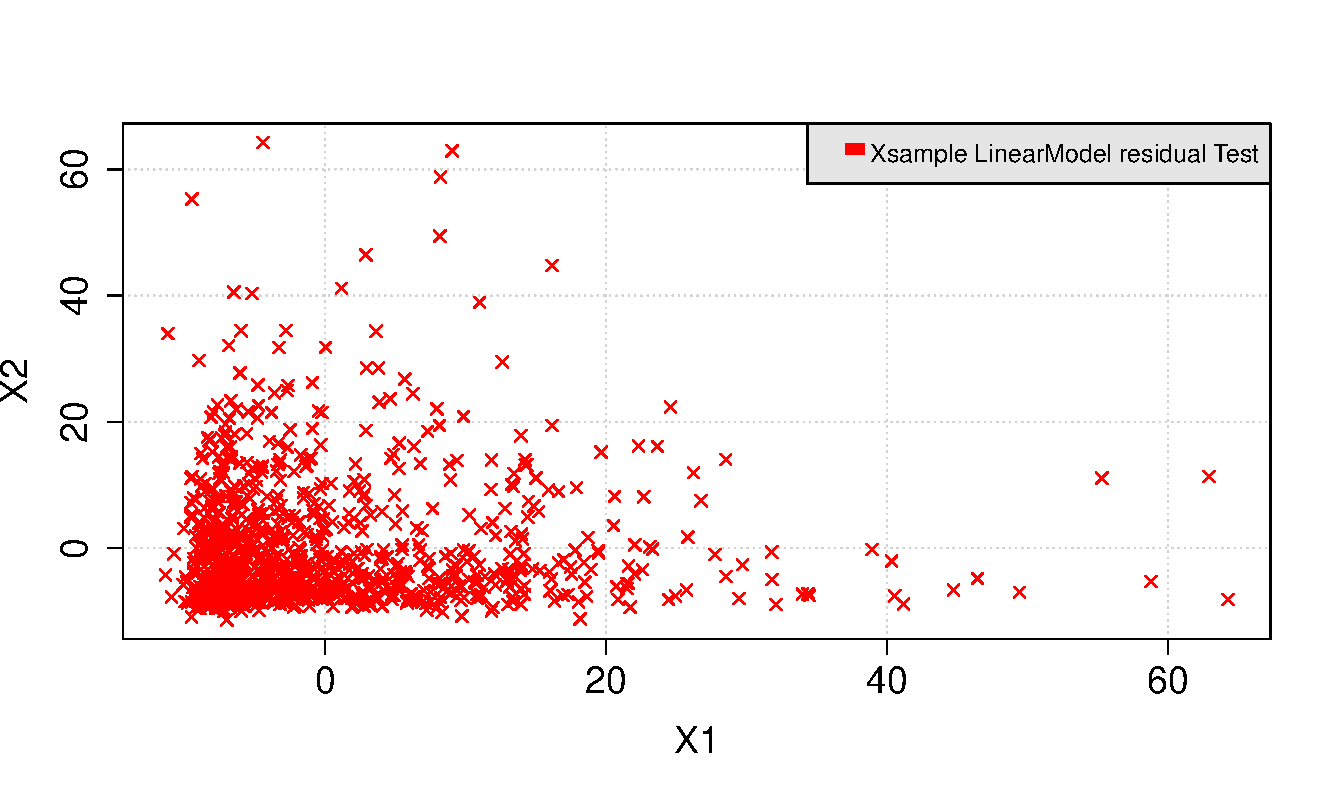
\includegraphics[scale=0.45]{Figures/WronglinearRegModelResidual.pdf}
  \end{center}

  \vspace{2mm}
}
{
}

\Methodology{
  Multiple linear regression can be used in step B "Quantifying Sources of Uncertainty". Having defined the vector $\underline{X}$ of input variables in step A "Specifying Criteria and the Case Study", linear regression allows to detect a linear type of dependency between uncertain variables.
  Such a relationship should in fact be taken in to account so as not to bias the results of step C "Propagation of Uncertainty".
}
            {
              As we have seen in the mathematical description, there is a consequent list of verifications that have to be carried to validate the linear model. In particular, underlying assumptions on the residuals are important to ensure the robustness of the average forecast. Detecting a non-conform behaviour of the residuals can also provide leads on transformations that could be carried out before applying linear regression (such as considering the logarithm of a variable instead of the variable itself).

              The following bibliographical references provide main starting points for further study of this method:
              \begin{itemize}
              \item Saporta, G. (1990). "Probabilités, Analyse de données et Statistique", Technip
              \item Dixon, W.J. \& Massey, F.J. (1983) "Introduction to statistical analysis (4th ed.)", McGraw-Hill
              \item NIST/SEMATECH e-Handbook of Statistical Methods, http://www.itl.nist.gov/div898/handbook/
                % \item D'Agostino, R.B. and Stephens, M.A. (1986). "Goodness-of-Fit Techniques", Marcel Dekker, Inc., New York.
              \item Bhattacharyya, G.K., and R.A. Johnson, (1997). "Statistical Concepts and Methods", John Wiley and Sons, New York.
                % \item Sprent, P., and Smeeton, N.C. (2001). "Applied Nonparametric Statistical Methods -- Third edition", Chapman \& Hall
                % \item Burnham, K.P., and Anderson, D.R (2002). "Model Selection and Multimodel Inference: A Practical Information Theoretic Approach", Springer
            \end{itemize}}
